\section{Data preprocessing}
\label{sec:data-preprocessing}

From all predictors in Table \ref{table:predictors}, only SSRD, STRD, TSR, TP and TCC are used 
because they are the most relevant predictors: SSRD, STRD and TSR can model the hypothetical maximum power 
output while TCC is relevant because it correlated with how much sun light actually get to the solar stations. 
Total precipitation is also important in the winter months since the solar stations can be covered with snow and no sun light gets through.
Since the Variables SSRD, STRD and TSR are all provided as accumulated fields, they first need to be decumulated.
This can be done by subtracting the value before the current value from the current value, for each day separately. 
Figure \ref{fig:strd-accumulated-vs-decumulated} shows both the accumulated and decumulated fields. 
A machine learning algorithm works better with the decumulated field since the decumulated field directly correlates 
with the power output of the solar plant.

Since machine learning models often work better with normalized data, it makes sense to normalize the predictors 
so that they take values in \([0,1]\) instead of \([0,\infty)\). 

\begin{figure}[h]%
    \centering
    \subfloat[\centering STRD accumulated]{{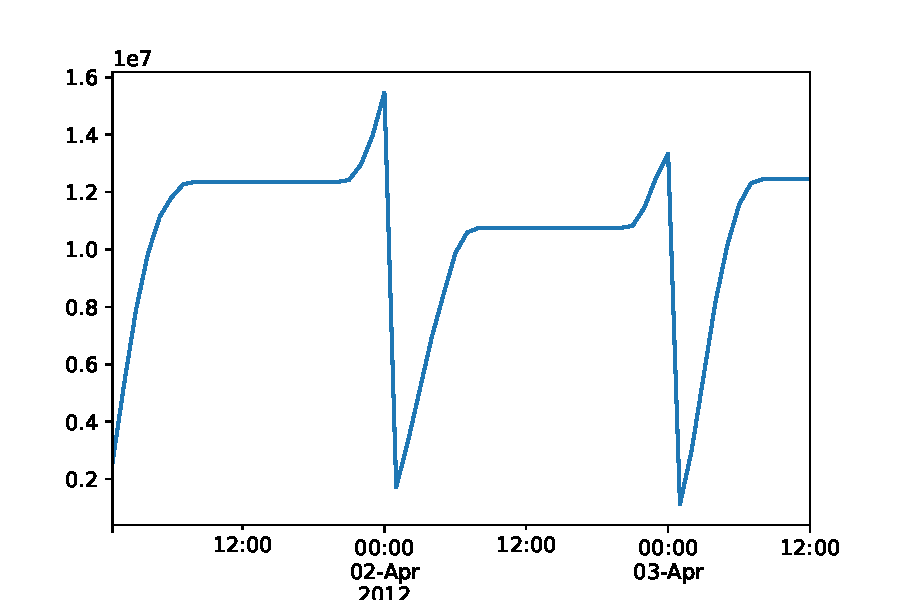
\includegraphics[width=7cm]{plots/strd_accumulated.pdf} }}%
    \qquad
    \subfloat[\centering STRD decumulated]{{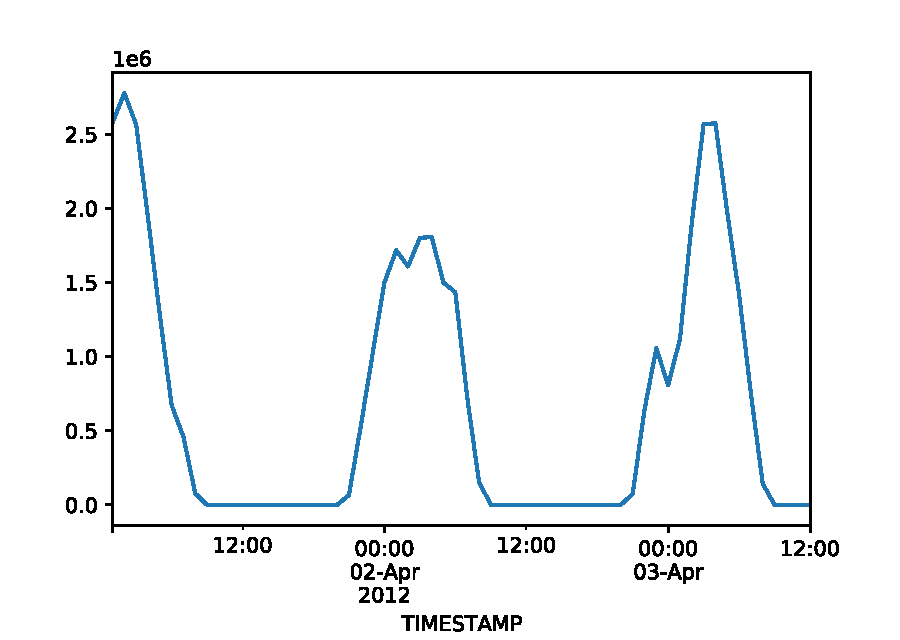
\includegraphics[width=7cm]{plots/strd_decumulated.pdf} }}%
    \caption[STRD accumulated vs. decumulated]{STRD accumulated vs. decumulated. 
    In order to get the actual data, we first need to subtract the previous point \(x_{t-1}\) from \(x_t\).}%
    \label{fig:strd-accumulated-vs-decumulated}%
\end{figure}